%%%%%%%%%%%%%%%%%%%%%%%%%%%%%%%%%%%%%%%%%%%%%%%%%%%%%%%%%%%%%%%%%%%%%%%%
% Plantilla TFG/TFM
% Escuela Politécnica Superior de la Universidad de Alicante
% Realizado por: Jose Manuel Requena Plens
% Contacto: info@jmrplens.com / Telegram:@jmrplens
%%%%%%%%%%%%%%%%%%%%%%%%%%%%%%%%%%%%%%%%%%%%%%%%%%%%%%%%%%%%%%%%%%%%%%%%

\chapter{Tecnologías}
\label{tecnologias}

    \section{Modelos}

        A continuación se presentarán los modelos con los que se ha experimentado para resolver este problema. 

        \subsection {Algoritmos Genéticos}
            Un \textit{Algoritmo Genético}, o \textit{Genetic Algorithm (GA)}, es un modelo que imita la evolución de las especies en el ámbito de la biología, con el objetivo de encontrar una solución potencialmente óptima a un problema mediante la evolución de un conjunto de soluciones denominadas individuos.\\

            El planteamiento de estos modelos consiste en evaluar los individuos pertenecientes a la población de la generación correspondiente para tomar el subconjunto de aquellas soluciones que mejor calidad ofrezcan (adaptación al medio) mediante una función heurística.\\

            Las funciones heurísticas son funciones aproximadas a una solución ideal del problema, debido a que todas las posibles combinaciones de los parámetros a optimizar genera un espacio de búsqueda de búsqueda exponencial (problema NP-hard), es necesario crear una aproximación mediante la función heurística para acotar el espacio de búsqueda.\\

            Para comprender el funcionamiento de los algoritmos genéticos es necesario analizar cada una de las fases que lo constituyen:
            
            \begin{enumerate}
                \item Inicialización de la Población:

                        En primer lugar es necesario generar los \textit{n} individuos de la población aleatoriamente. Cada uno de estos individuos está formado por el conjunto de parámetros que son objeto de optimización \ref{InitialPopulation}.

                        \begin{figure}[h]
                            \centering
                            \includesvg[inkscapelatex=false]{archivos/GA/InitialPopulation}
                            \caption{Inicialización de la población.}
                            \label{InitialPopulation}
                        \end{figure}

                \item Evaluación de Población:

                        Es la primera fase del proceso iterativo del algoritmo genético. En él, cada uno de los individuos pertenecientes a la población son evaluados mediante la función \textit{fitness} para obtener el \textit{score} de cada individuo de la población actual.

                \item Selección de Padres:

                        Una vez evaluados los individuos de la población, se procede a seleccionar aquellos padres que mejor \textit{score} han obtenido para crear nuevas soluciones a partir de éstos. Existen distintas técnicas de selección, como por ejemplo escoger aquellos \textit{n} mejores padres de la población o técnicas basadas en métodos probabilísticos, para que aquellos individuos que menos puntuación logren, tengan alguna probabilidad de ser elegidos para la generación de nuevas soluciones. Este tipo de técnicas se utilizan para aumentar la diversidad en la pobĺación y evitar caer en soluciones acotadas a mínimos locales del problema. Se puede ver el proceso de cómo son seleccionados los padres en función de su \textit{fitness} en la figura \ref{FitnessFunction}.

                        \begin{figure}[h]
                            \centering
                            \includesvg[inkscapelatex=false]{archivos/GA/FitnessFunction}
                            \caption{Selección de padres candidatos.}
                            \label{FitnessFunction}
                        \end{figure}

                \item Cruzamiento:

                        Una vez seleccionados los padres es necesario que intercambien información entre ellos para dar lugar a nuevos individuos, este proceso de herencia de información es posible realizarlo aplicando distintas filosofías; seleccionar un punto o posición de cruzamiento a lo largo del vector de los padres y combinar ambos padres, o escoger aleatoriamente las posiciones de los parámetros de ambos padres y se combinen para dar lugar a la solución generada \ref{ParentsMatingMutationImage}.

                        \begin{figure}[h]
                            \centering
                            \includesvg[inkscapelatex=false]{archivos/GA/ParentsMatingMutation}
                            \caption{Mutación de hijos.}
                            \label{ParentsMatingMutationImage}
                        \end{figure}

                \item Mutación:

                        Cuando los padres seleccionados son combinados para dar lugar a los candidatos de la nueva generación, es importante aplicar un proceso de mutación entre éstos debido a la necesidad de generar diversidad en la población. Si se combina la misma información entre generaciones, se corre el riesgo de converger prematuramente a un mínimo local del espacio de búsqueda. Por este motivo se introduce el concepto de mutación, que consiste en aplicar una modificación aleatoria sobre alguno de los parámetros de los individuos generados para poder ampliar el espacio de soluciones. 
            \end{enumerate}

            Cada una de las fases enumeradas anteriormente se repite de forma iterativa entre generaciones hasta que se cumpla alguna condición de parada, como establecer un umbral mínimo del \textit{score} de las soluciones, o fijar un número específico de iteraciones que se ejecutarán en el algoritmo.\\


            A continuación enumeraremos los parámetros con los que configurar un algoritmo genético. Dependiendo del tipo de algoritmo utilizado es posible encontrar distintos parámetros con los que inicializar el algoritmo, sin embargo estos son los más extendidos:


            \begin{itemize}

                \item Tamaño de la población:

                Ees el número de individuos que sobrevivirán entre iteraciones, es decir, los individuos que se tratarán de mejorar a lo largo de las ejecuciones. En los experimentos de este trabajo Sección 5 se han inicializado 100 individuos, cada uno de ellos con 4 hiperparámetros del algoritmoo \textit{XGBoost} a optimizar.

                \item Número de iteraciones:

                Es el número generaciones que evolucionarán en el algoritmo. Habitualmente un mayor número de iteraciones permite una mayor precisión de los resultados a costa de invertir recursos computacionales, debido a que existen mayores probabilidades de que los individuos evolucionen. En los experimentos se han usado el mismo número de iteraciones para cada uno de los algoritmos. Esto provoca que el tiempo de ejecución entre algoritmos varíe debido a su propia naturaleza.

                \item Probabilidad de cruce:

                Probabilidad con la que dos padres intercambian su información entre sí para dar lugar a un nuevo individuo hijo.

                \item Probabilidad de mutación:

                Indica la probabilidad con la que cada hiperparámetro puede variar su valor, es decir, con una probabilidad de 0.5, cada hiperparámetro de un individuo hijo tiene un 50 por ciento de probabilidades de modificar su valor. Se establece además un rango de posibles valores en los cuales un párámetro de un individuo puede mutar, es decir, se definen unos valores máximos y mínimos en los que el parámetro mutará y se escoge un valor aleatorio dentro del rango. De esta forma si muta un mismo parámetro para varios individuos de la generación, esta condición se asegurará de que las variaciones aplicadas a cada uno de ellos estén controladas y sean distintas para cada uno de ellos.

            \end{itemize}


        \subsection {XGBoost}

            
            \textit{Extreme Gradient Boosting Algortihm} (\textit{XGBoost}) es una libería open-source que implementa algoritmos \textit{ML Ensembles de tipo Boosting}. Se trata de uno de los algoritmos más importantes de los últimos años, logrando un rendimiento diez veces mayor a otras soluciones populares en una misma máquina y llegando a las primeras posiciones en numerosos retos propuestos en \textit{Kaggle} \cite{XGBoostTutorial}.\\

            XGBoost se basa en los modelos \textit{Ensemble Boosting} de los algoritmos de \textit{ML}, de ahí su nombre \textit{Gradient Boosting}. La técnica \textit{Boosting} se basa en construir un modelo robusto (\textit{strong learner}) combinando una serie de modelos débiles (\textit{weak learners}) \cite{NvidiaXGBoost}.\\


            Concretamente \textit{XGBoost} implementa \textit{Gradient Boosting Decision Trees (GBDT)}, que es un algoritmo similar a los \textit{Random Forest}, y es utilizado tanto para clasificación como para regresión.\\

            La diferencia principal de los \textit{Random Forest} con respecto a \textit{XGBoost} radica en la diferencia en la que los \textit{Ensembles Bagging} calculan las predicciones. Los algoritmos de tipo \textit{Bagging} construyen $n$ modelos de las mismas características pero entrenados con distintos ejemplos muestreados desde el conjunto de entrenamiento, y construye un modelo final predictivo en el que la salida predecida será la combinación de la predicción de cada uno de los modelos individuales, sobre sus resultados se pueden aplicar distintas estrategias para escoger la predicción agregada de éstos (como realizar la media de las predicciones, escoger la predicción más frecuente de los modelos individuales, etc).\\

            En el caso de los \textit{Ensembles Boosting} la idea es combinar secuencialmente modelos (\textit{Árboles de decisión}) de tal forma que su objetivo es minimizar los residuos de los árboles generados anteriormente, en lugar de crear una predicción conjunta entre todos ellos como era el caso de los \textit{Ensembles Bagging}, y utiliza el método de \textit{Gradient Descent} para minimizar estos residuos.\\


            En la figura \ref{XGBoostFlowImage} se puede observar cómo se van construyendo los árboles clasificadores y cómo cada árbol minimiza el residuo producido por el árbol anterior.\\


            \begin{figure}[h]
                \centering
                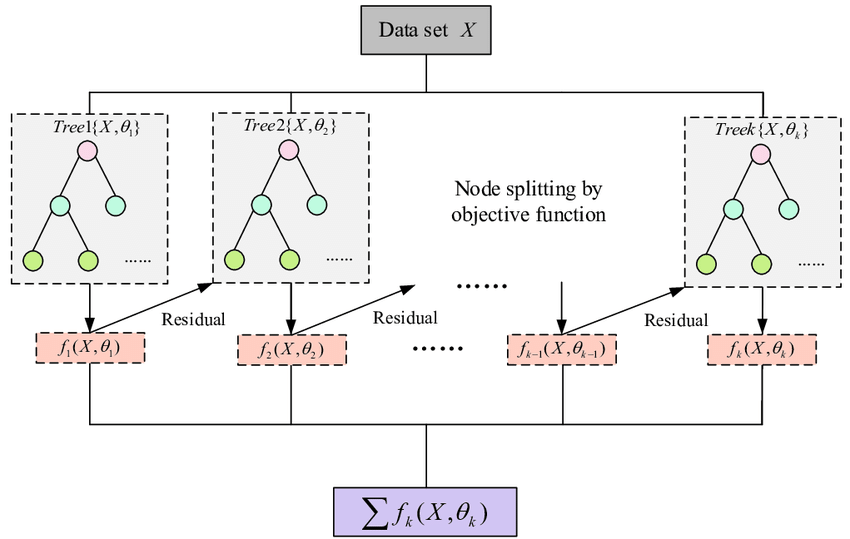
\includegraphics[width=10cm]{archivos/XGBoostFlowImage}
                \caption{Degradation state recognition of piston pump based on ICEEMDAN and XGBoost(FIG3). Proceso de optimización de XGBoost.}
                \label{XGBoostFlowImage}
             \end{figure}

            
            Además, \textit{XGBoost} aplica técnicas de regularización en su función de pérdida, de tal forma que reduce la influencia individual de cada árbol generado y de sus hojas para poder dar lugar a posteriores árboles que consigan mejorar el modelo, evitando de esta manera el sobreajuste u \textit{overfitting}.



        \subsection {Redes Neuronales Convolucionales (CNN)}

            Las Redes Neuronales Convolucionales tratan de imitar el comportamiento del sistema nervioso para identificar patrones en los datos de entrada.\\

            Para entrenar a una \textit{CNN} es necesario hacerlo mediante ejemplos etiquetados, ya que este tipo de redes se basa en el aprendizaje supervisado. Es decir, durante el proceso de entrenamiento se comparará la salida de las predicciones de la última capa con la salida conocida, y se calculará la entropía cruzada entre las distribuciones  para optimizar los pesos de las capas mediante el método \textit{Descenso por Gradiente} \textit{(Backward Propagation)}.\\


            A modo de comprensión, se muestra la arquitectura de una \textit{NN}, donde se pueden observar las conexiones entre cada capa de la red y sus salidas en la figura \ref{NNImage}. Existe una capa de entrada inicial \textit{input layer} que corresponde a cada una de las características del ejemplo de entrada (en el caso de imágenes se trata de cada uno de los píxeles). Cada una de las características de la capa de entrada se conecta con cada una de las neuronas primera capa oculta \textit{hidden layer} a través de conexiones denominadas pesos \textit{weights} que son los que serán aprendidos en la red con el objetivo de encontrar patrones entre las características mediante el método de \textit{Descenso por Gradiente} o \textit{Gradient Descent (GD)}.\\


            Esta metodología se aplica para cada una de las \textit{hidden layers} presentes en la arquitectura hasta la última capa, para que la red aprenda patrones entre las distintas salidas de cada capa hasta llegar a una función \textit{SoftMax} que dictará la clase predicha en base a la salida de la capa final, u \textit{output layer}.\\

            \begin{figure}[h]
                \centering
                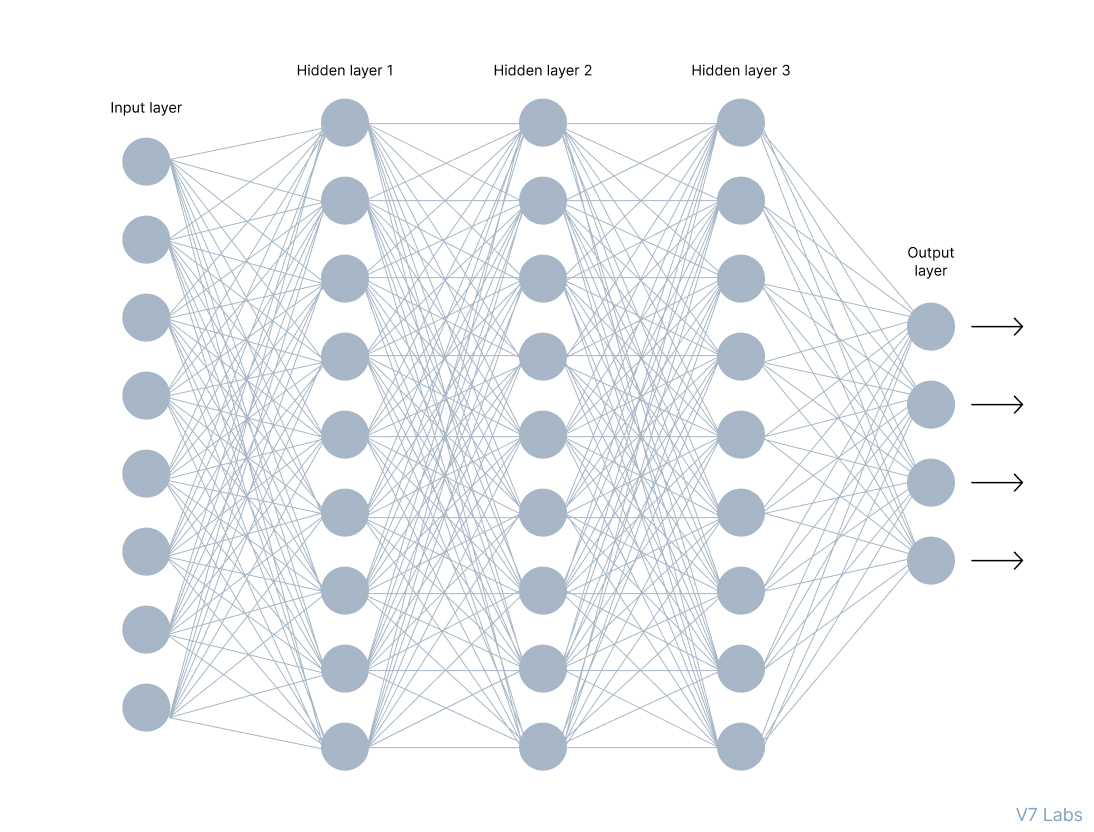
\includegraphics[width=10cm]{archivos/NNImage}
                \caption{https://www.v7labs.com/blog/neural-networks-activation-functions. Arquitectura de una Red Neuronal.}
                \label{NNImage}
             \end{figure}



            Antes de entrar en el detalle de la implementación de las \textit{CNN} es necesario introducir los siguientes conceptos comunes a todas las \textit{NN} para la posterior comprensión de las arquitecturas:


            \begin{itemize}

                \item Función de activación:

                    Las funciones de activación son las encargadas de decidir si una neurona es activada o no en función de la entrada a esta función, es decir, basándose en los datos de entrada a la función, ésta decidirá si este input producirá un determinado \textit{output} a la salida de ella. Esta función suele situarse en la salida de cada capa de la red para decidir si una determinada neurona de la siguiente capa se activará o no.

                    Existen distintos enfoques en lo que respecta a las funciones de activación, como 

                    En el caso de este proyecto, se utilizará la función de activación \textit{Rectified Linear Unit (ReLU)}, que se comporta devolviendo el valor $0$ para aquellas entradas que sean negativas y el valor original para aquellas que sean positivas, se puede apreciar el comportamiento en la figura \ref{RELUImage}.

                    \begin{center}
                        $f(x) = \left\{
                                       \begin{array}{lr}
                                         0 & \text{if } x<=0\\
                                         x & \text{if } x>0
                                       \end{array}
                                \right.$
                    \end{center}

                    \begin{figure}[h]
                        \centering
                        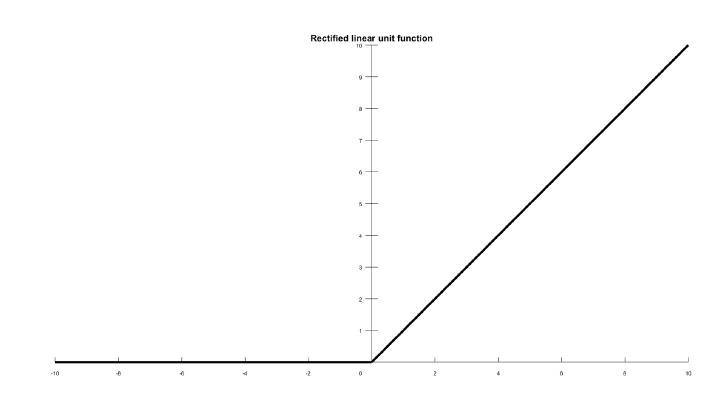
\includegraphics[width=10cm]{archivos/CNN/RELUImage}
                        \caption{https://www.researchgate.net/journal/Transport-in-Porous-Media-1573-1634. Función ReLU}
                        \label{RELUImage}
                     \end{figure}


                \item Entropía:

                    La entropía sobre una varible aleatoria $X$ es el grado de incertidumbre producido en base a los posibles valores que puede tomar como respuesta, es decir, a mayor entropía de una variable aleatoria $X$, existe mayor grado de incertidumbre sobre ella. La entropia $H(X)$ se calcula en base a la siguiente fórmula:

                    \begin{center}
                        $H(X) = -\sum_{i = 1}^n p(x_i) \log_2 p(x_i)$
                    \end{center}

                    Donde $x_i$ es cada uno de los posibles valores que puede tomar la variable como respuesta y $p(x_i)$ es la probabilidad de obtener dicho valor. Por lo tanto, es deseable mantener distribuciones con un grado de entropía bajo, ya que existirá menos incertidumbre en ella.


                \item Softmax:

                    Se trata de la generalización en forma multidimensional de la función logística o \textit{logistic function}. Softmax es una función que permite la transformación de un vector de números reales a una distribución de probabilidad. Esta función se suele aplicar como capa de activación en el último nivel en las \textit{NN}, representando la probabilidad de que la salida de la red pertenezca a cada una de las $K$ clases posibles en el modelo \cite{Softmax}. 

                    Esto se debe a que normalmente los componentes de la salida de la última capa de una red neuronal (denominados como \textit{logits}) son el resultado de la predicción en forma de números reales no normalizados, por lo tanto pueden ser mayores que $1$ e incluso negativos. La función permite calcular la distribución de probabilidad en base a estos \textit{logits} y calcular la probabilidad de pertenencia a cada una de las $K$ clases que componen el modelo mediante la siguiente fórmula:


                    \begin{center}
                        $\sigma(z_i) = \frac{e^{z_{i}}}{\sum_{j=1}^K e^{z_{j}}} \ \ \ for\ i=1,2,\dots,K$
                    \end{center}


                    Esta función es continua y diferenciable, por lo que es posible aplicar el método \textit{GD} para actualizar los valores de los pesos de la red neuronal en las capas anteriores gracias a estas propiedades que permiten la derivabilidad de la función.


                \item Cross-Entropy:

                    El objetivo de cross-entropy es minimizar la función de pérdida (\textit{log loss}) comparando la probabilidad de la clase predicha con respecto a su valor verdadero. Al aplicar una penalización logarítmica, las probabilidades de las clases que más disten respecto a su valor verdadero se verán más acentuadas \cite{Cross-Entropy}.

                    \begin{center}
                        $L_{CE} = -\sum_{i = 1}^n y_i \log_2(p_i)$
                    \end{center}

                    Donde $n$ es el número de clases a predecir, el valor $y_i$ es la etiqueta de la clase verdadera, y $p_i$ es la probabilidad de que la muestra actual pertenezca a la clase $i$.

                    \begin{figure}[h]
                        \centering
                        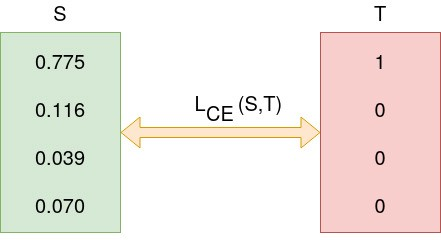
\includegraphics[width=7cm]{archivos/CNN/CrossEntropy}
                        \caption{https://towardsdatascience.com/cross-entropy-loss-function-f38c4ec8643e}
                        \label{CrossEntropyImage}
                     \end{figure}

                \item BackPropagation:

                    En el proceso de entrenamiento de la \textit{CNN} es necesario actualizar los pesos de las capas ocultas con el objetivo de minimizar la cross-entropy total del modelo. Para minimizar este valor se utiliza el método \textit{GD}, algoritmo de optimización que maximiza el valor de una función siempre y cuando ésta sea continua diferenciable.

                    Gracias a las propiedades de la función \textit{Softmax} es posible utilizar \textit{GD} para calcular la derivada de la función de pérdida respecto de cada uno de los pesos de las capas intermedias de la red y actualizar cada uno de ellos con el objetivo de minimizar la función de pérdida.

                \item Batch Normalization:

                    El proceso de entrenamiento de una red neuronal puede ser costoso, ya que existen una gran cantidad de parámetros para cada capa que son optimizados durante el proceso de entrenamiento. Esto hace que este proceso sea demasiado sensible a los parámetros inicializados en el inicio del entrenamiento de la red, como es el ejemplo de establecer una tasa de aprendizaje \textit{learning rate} muy baja para poder converger. Esto hace que el entrenamiento sea muy lento, por lo que es necesario transformar los datos de entrada a la entrada de la capa, o lo que es lo mismo, normalizar las entradas para cada mini-batch (subconjuntos de datos de entrenamiento con el que se entrena la red en cada época \textit{epoch}).


                    El método \textit{Batch Normalization} \cite{BatchNormalization} normaliza los datos de tal forma que permite utilizar tasas de aprendizaje mayores además de actuar como regularizador, reduciendo así el número de capas \textit{Dropout} que existan en la arquitectura.

            \end{itemize}


            A contiuación definiremos los parámetros específicos aplicados a las \textit{CNNs}:

            \begin{itemize}

                \item Kernels:

                    Son las estructuras que se encargan de realizar la convolución. Los kernels son matrices de pesos unidimensionales ($1 \times n$) o bidimensionales ($n \times m$)dependiendo del tipo de convolución que se esté aplicando (Convolución 1-D o Convolución 2-D), y se encargan de proyectar las posiciones de la matriz de entrada que correspondan en instante de la convolución en un mapa de características (\textit{feature map}), que será el input de la siguiente capa de la red. De esta forma, los kernels permiten inferir patrones en la matriz de entrada en gracias a la actualización de sus pesos. En función de la profundidad de la capa, los kernels podrán encontrar patrones más simples (capas más superficiales de la red) o más complejos (capas más profundas de la red) debido a que la entrada a cada capa es una convolución (aplicación del filtro) de las capas anteriores.

                    Un kernel realiza el producto escalar de sus pesos con respecto a las posiciones de la matriz de entrada (imagen o \textit{feature map}) que colisionen en ese momento con el kernel, generando un nuevo \textit{feature map} de menor dimensión, a menos que se utilice la técnica de \textit{Padding} \cite{Kernels}.
                     
                \item Filtros:

                    Un filtro no es más que una agrupación de kernels, siempre tendrán una dimensión mayor que la definida para el kernel. Por ejemplo, si disponemos de un kernel unidimensional ($1 \times n$), el filtro contendrá $k$ kernels de ($1 \times n$) en la capa convolucional definida \cite{FiltersFeatureMaps}

                \item Strides:

                    Son los saltos producidos por un kernel en cada etapa de la convolución, dependiendo si la convolución es dimensional o bidimensional, el stride constará de una dimensión ($i$), es decir, los pasos hacia la derecha en la imagen, o de dos dimensiones ($i, j$), los pasos hacia la derecha y hacia abajo en la imagen.

                    \begin{figure}[h]
                        \centering
                        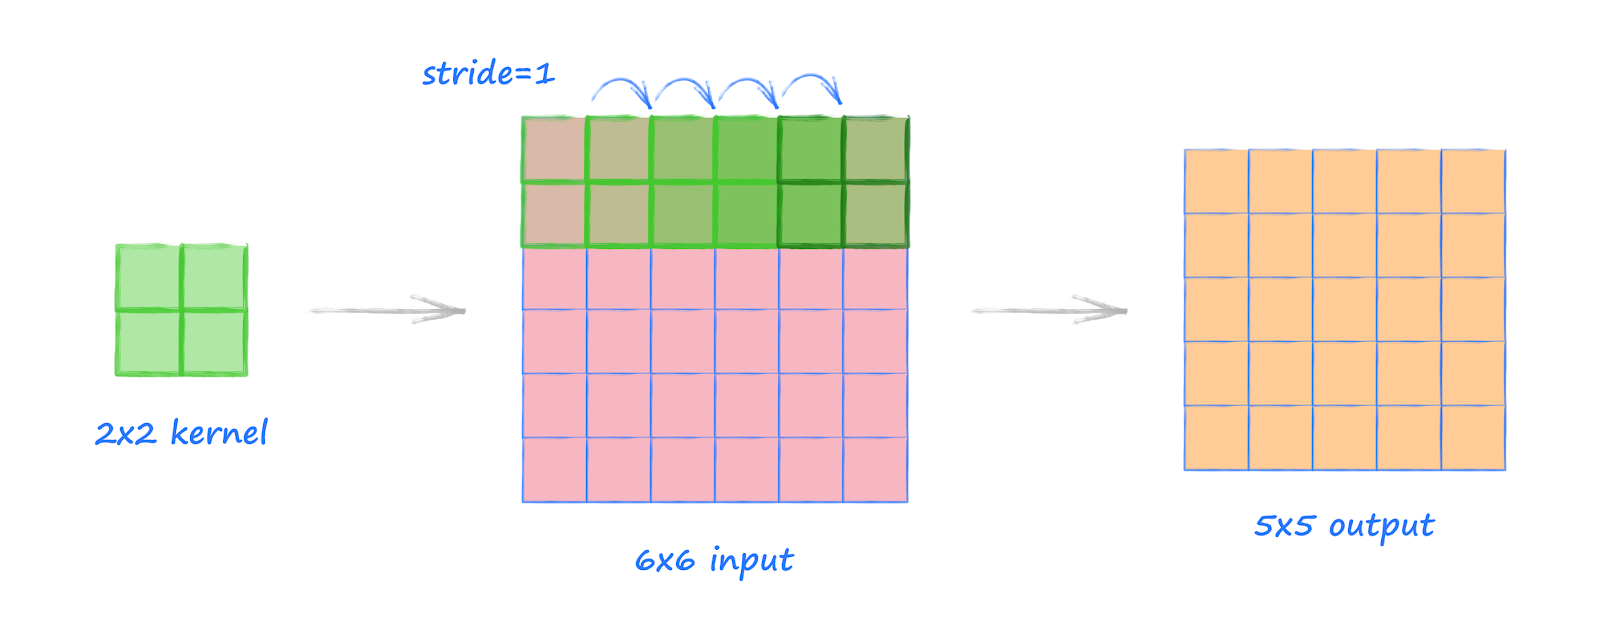
\includegraphics[width=10cm]{archivos/CNN/Stride}
                        \caption{http://makeyourownneuralnetwork.blogspot.com/2020/02/calculating-output-size-of-convolutions.html}
                        \label{StrideImage}
                     \end{figure}

                \item Padding:

                    El padding es un método utilizado para incrementar la dimensionalidad de la entrada de la capa debido el desvanecimiento de los valores posicionados en zonas comprometedoras una vez aplicada la convolución. Estas posiciones son aquellas en las que el filtro de la convolución pasaría una única vez en caso de no aplicar \textit{padding}.\\

                    El \textit{padding} es el proceso de generar celdas artificiales inicializadas con valor \textit{0} que permiten que el filtro convolucional sea aplicado en su totalidad en la posición de estas zonas comprometedoras, manteniendo la información de los límites de la imagen. De otra forma ĺos valores de estos extremos se desvanecerían a medida se incrementa la profundidad de la red (número de capas) con respecto al resto de valores de la matriz.\\

                    \begin{figure}[h]
                        \centering
                        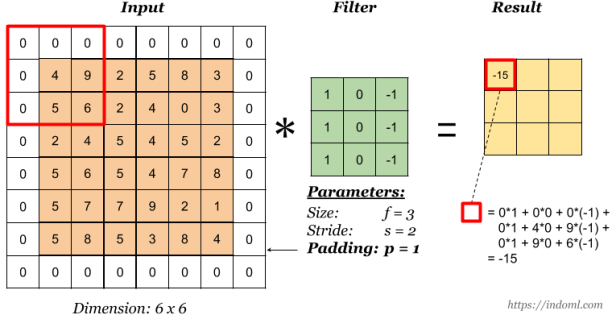
\includegraphics[width=10cm]{archivos/CNN/padding}
                        \caption{https://indoml.com/2018/03/07/student-notes-convolutional-neural-networks-cnn-introduction/}
                        \label{PaddingImage}
                     \end{figure}


                \item Función de activación:


                    En el caso de las redes neuronales convolucionales, la forma de aplicar la función de activación 



                    \begin{figure}[h]
                        \centering
                        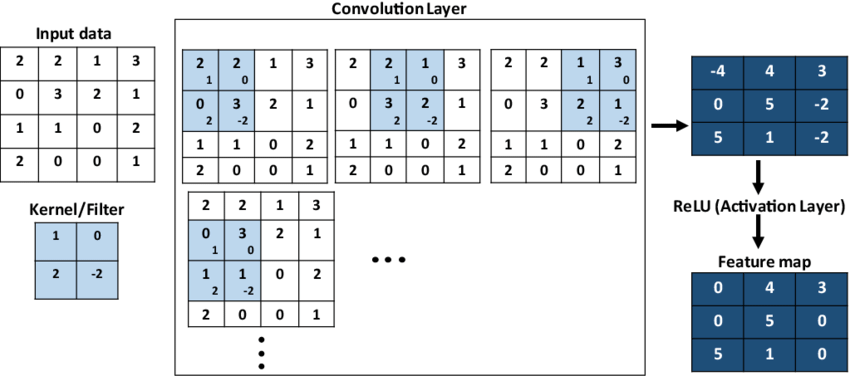
\includegraphics[width=10cm]{archivos/CNN/CNNRELUImage}
                        \caption{https://www.researchgate.net/journal/Transport-in-Porous-Media-1573-1634}
                        \label{CNNRELUImage}
                     \end{figure}

            \end{itemize}

            En el proceso de entrenamiento de las \textit{CNNs} cada uno de los valores de los kernels son optimizados mediante el método \textit{GD}, de tal forma que los pesos de cada capa son actualizados gracias a la derivabilidad de la función de pérdida.

            !!!!!\cite{KL-Divergence}!!!!!

            Una vez definidos los pasos que sigue el entrenamiento de una \textit{NN} y las características propias de las \textit{CNNs}, podemos hacer distinción entre los dos enfoques distintos de \textit{CNNs} que se han aplicado en este proyecto. Cabe mencionar que el funcionamiento de ambas \textit{CNNs} únicamente difiere en el tamaño del \textit{kernel} y la forma en la que éste se desplaza debido a dimensionalidad de éste.


            \subsubsection{Unidimensionales (Conv-1D)}
            
                Una \textit{Red Neuronal Convolucional de 1 Dimensión}, o \textit{Convolutional Neural Network 1-Dimensional (CNN-1D)}, es un tipo de red convolucional que utiliza kernels \textit{(filters)} que son aplicados a las imágenes de entrada con el objetivo encontrar ciertas características en ellas.\\

                Las complejidad computacional de las \textit{CNN-1D} es mucho más simple que las \textit{CNN-2D}, además, estas redes se han demostrado ser más efectivas en distintos campos con respecto a las \textit{CNN-2D}, como en técnicas de análisis de señales. La baja carga computacional de esta arquitectura la hace atractiva para aplicarla en tiempo real en dispositivos con pocos recursos como teléfonos móviles \cite{Conv1D_Survey}.\\


                El resultado de este proceso es la proyección del filtro sobre un espacio dimensional denominado mapa de caracerísticas \textit{(feature maps)}. Este filtro se utiliza para convolucionar los feature maps de la capa anterior \cite{FiltersFeatureMaps} o de la imagen de entrada si se trata de la primera capa de la red.
                

                \begin{figure}[h]
                    \centering
                    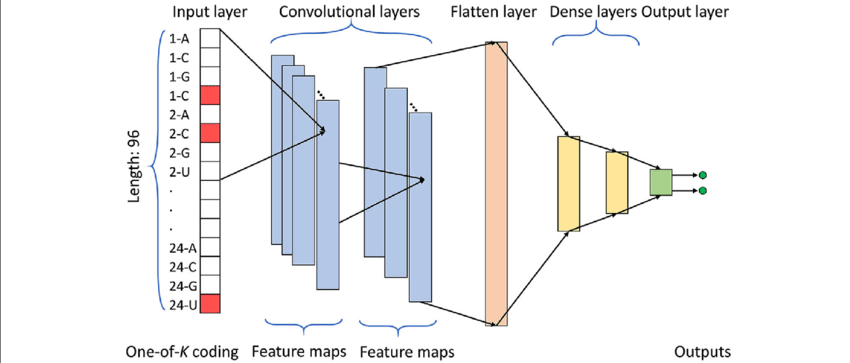
\includegraphics[width=15cm]{archivos/CNN/1D/1CNNArchImage}
                    \caption{https://www.researchgate.net/publication/329201018/figure/fig2/AS:697400008138753@1543284527161/The-architecture-of-our-1D-CNN-model-This-model-consists-of-two-convolutional-layers.png}
                    \label{1CNNArchImage}
                \end{figure}


                Al ser una arquitectura unidimensional, el \textit{kernel} tendrá que tener un tamaño ($1 \times n$).

                \begin{figure}[h]
                    \centering
                    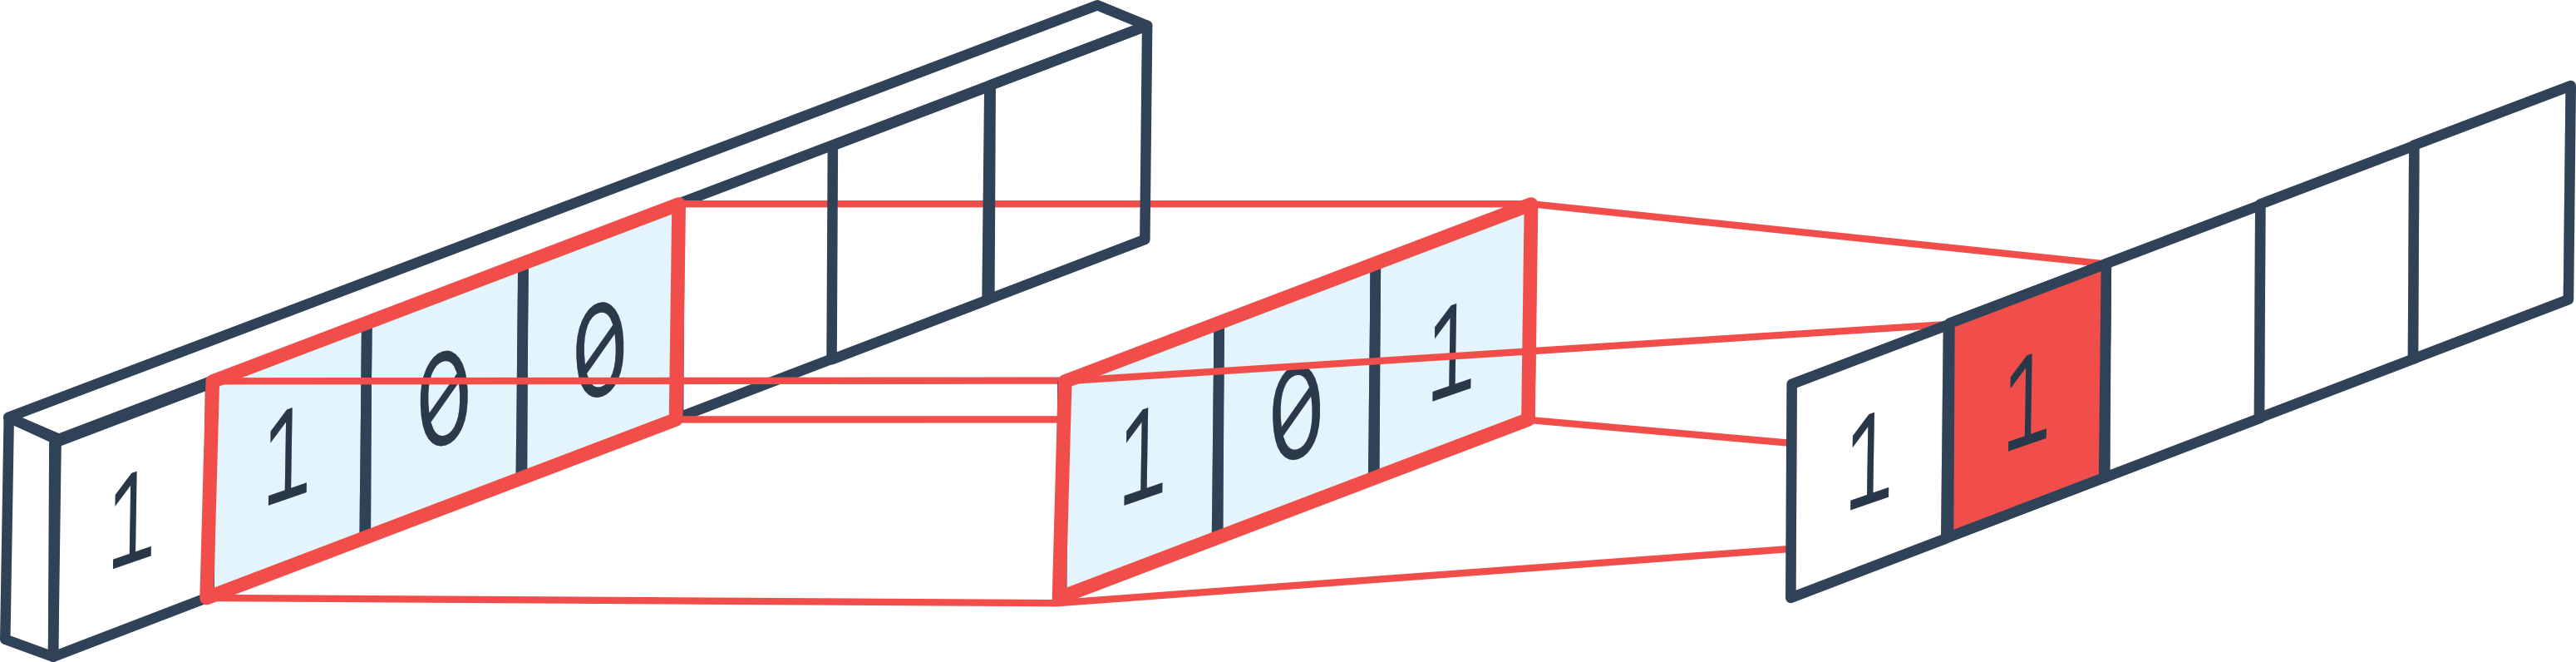
\includegraphics[width=7cm]{archivos/CNN/1D/1DConvolution}
                    \caption{https://peltarion.com/knowledge-center/documentation/modeling-view/build-an-ai-model/blocks/1d-convolution Observamos la entrada de la red (izquierda) a la que se le aplica un kernel (en el centro) que resulta en la convolución de un mapa de características (derecha).}
                    \label{1DConvolutionImage}
                \end{figure}

                
            \subsubsection {Bidimensionales (Conv-2D)}
                Otra de las técnicas convolucionales utizadas en este documento son las \textit{Redes Neuronales Convolucionales de 2 Dimensiones}, o \textit{Convolutional Neural Networks 2-Dimensional (CNN-2D)}. Al igual que en el caso de las \textit{CNN-1D}, el filtro se aplica sobre el input de la capa, resultando en \textit{feature maps}, sin embargo en este caso \textit{kernel} será de bidimensional por ser una convolución de dos dimensiones, es necesario especificar el tamaño de la matriz que recorrerá la matriz pasada como input a la capa correspondiente.

                \textit{}

        \subsection {KNN}

            El algoritmo \textit{K vecinos más próximos}, o \textit{K-Nearest Neighbors (kNN)} \cite{KNN}, es una técnica de aprendizaje supervisado ampliamente utilizada para tareas de clasificación y regresión, es uno de los algoritmos más básicos de \textit{ML} y tiene una gran importancia en el campo de la \textit{Ciencia de Datos} debido a su simplicidad de implementación y a su interpretabilidad.\\

            El algoritmo \textit{KNN} asume que muestras con características parecidas deben pertenecer a la misma clase. O lo que es lo mismo, muestras parecidas deben estar cercanas en el espacio dimensional.\\

            Esta técnica se basa en representar las muestras de un conjunto de datos en base a sus características en un espacio n-dimensional y clasificar la muestra correspondiente como la clase mayoritaria al calcular la distancia de dicha muestra a los $k$ vecinos más próximos. Normalmente la distancia empleada es la \textit{Euclídea}, aunque es posible calcular otras distancias como \textit{Manhattan} o \textit{Chebyshev}.\\
            
            A medida que se incrementan las dimensiones del espacio resulta más costoso computacionalmente calcular distancias entre los puntos.\\


            Por lo tanto, el único parámetro a configurar es el número de vecinos más cercanos que se calculará en base al punto que queramos clasificar, en la figura \ref{KNNImage} se muestra un ejemplo de un problema de clasificacíón aplicando distintos valores al parámetros $k$.

            \begin{figure}[h]
                \centering
                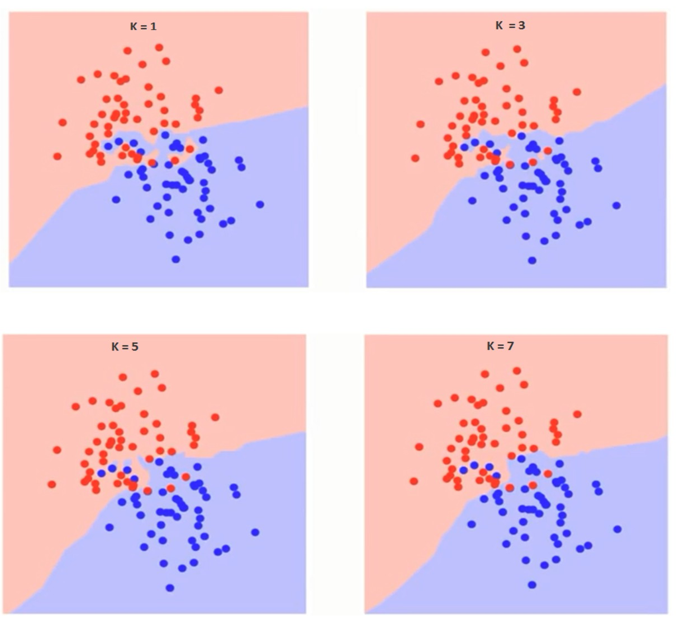
\includegraphics[width=10cm]{archivos/CNN/KNN/KNNImage}
                \caption{https://forum.huawei.com/enterprise/es/data/attachment/forum/202108/20/150033de3l4nyvmcbozh14.png?KNN3.png KNN aplicado con distintos valores de $k$}
                \label{KNNImage}
            \end{figure}

            

    \section{Especificaciones técnicas}

        En esta sección detallaremos las herramientas que han sido utilizadas para poder realizar este proyecto.


        \subsection{Herramientas utilizadas}
            Para el desarrollo de este proyecto se ha hecho uso de los siguientes programas:

            \begin{itemize}
                \item Lenguaje de programación:
                    \subitem Python: lenguaje de programación interpretado de nivel alto multiparadigma. La versión empleada para el desarrollo del proyecto ha sido 3.9.11.
                \item Liberías: Se enumerarán las librerías 
                    \subitem Pandas: libería que provee de herramientaas que permiten el análisis y la manipulación de datos. La versión utilizada para este proyecto es la 1.3.5 \cite{Pandas}. 
                    \subitem Tensorflow: libería utilizada para la implementación de redes neuronales permitiendo su ejecución. Este proyecto se basa en la versión 2.8.0 \cite{Tensorflow}.
                    \subitem Sklearn: librería que contiene múltiples modelos predictivos implementados, basado en NumPy, SciPy y Matplotlib. La versión configurada para este proyecto es 1.0.2 \cite{Scikit-Learn}.
                    \subitem XGboost: paquete que contiene la implementación del algoritmo XGBoost, además de múltiples configuraciones como la ejecución en \textit{CPU, GPU y GPU paralelizada}. La importación de esta librería ha sido en base a la versión 1.5.0 \cite{XGBoostLibrary}.
                \item Software:
                    \subitem CUDA: plataforma de computación paralelizada que permite la ejecución de código en \textit{GPU}, esto permite que las redes neuronales puedan entrenarse con mayor rapidez que en \textit{CPU} debido a la velocidad con la que se realizan las operaciones orientadas a datos en las tarjetas gráficas. Se ha utilizado la versión 11.6 \cite{CUDA}. 
                    \subitem Anaconda: distribución open-source que ofrece la flexibilidad de mantener varios entornos con distintas configuraciones y versiones de distinas librerías, facilitando además la migración entre equipos. La versión utilizada ha sido la 4.12.0 \cite{Anaconda}.
                    \subitem Jupyter Notebook: entorno interactivo que permite la creación, edición y ejecución de notebooks de forma local y remota. La versión utilizada para el desarrollo de este proyecto ha sido la 6.4.10 \cite{JupyterNotebook}.
                    \subitem Jupyter Lab: interfaz de nueva generación que convive con el entorno Jupyter Notebook, ofrece numerosas funcionalidades como es la navegación entre distintos repositorios dentro de la interfaz. La versión instalada para la realización del proyecto ha sido la 3.3.2 \cite{JupyterLab}.
                    \subitem MiKTeX:
                    \subitem DiagramsNet: plataforma utilizada para la confección de figuras mostradas en este documento \cite{DiagramsNet}. 
                    \subitem Google Meets: plataforma utilizada para realizar reuniones semanales con el tutor \cite{GoogleMeet}.
                \item Sistemas de control de versiones:
                    \subitem Github: repositorio donde tener un control de las versiones del desarrollo \cite{Github}.
                    
            \end{itemize}


        \subsection{Especificaciones del servidor}
            Los experimentos de este artículo se han realizado bajo un servidor con CPU \textit{Dual AMD Rome 7742} (128 cores) y contando con una GPU \textit{DGX NVIDIA A100} de  40 GigaBytes (\textit{GB}).
            